\section{Teilchen in Materie}
\subsection{Bethe-Bloch}
Geladene Teilchen die sich durch Materie bewegen verlieren durch Interaktionen mit den Atomen an Energie. Diese Interaktionen umfassen Bremsstrahlung bei hohen Energien, Ionisation bei mittleren Energien und Anregung von Atomen bei geringen Energien. Der Energieverlust in Abhängigkeit von der Energie des Teilchens ist in Abb. \ref{fig:bethe} dargestellt.\comment{Rpp2012-rev-passage-particles-matter}Für schwere geladene Teilchen, wie z.B. das Muon wird der Energieverlust durch Ionisation durch die Bethe-Bloch Formel beschrieben.
\begin{align*}
- \left<\frac{dE}{dx}\right> =  K\cdot \frac{Z}{A}\frac{z^2}{\beta^2} \cdot \left[ \frac12\ln \left(\frac{2m_ec^2\cdot\beta^2\cdot\gamma^2 \cdot T_{max}}{I^2}\right) - \beta^2 - \frac{\delta(\beta\gamma)}{2}\right]
\end{align*} 
Diese Formel hängt lediglich von der Ladung $z$ und der relativistischen Geschwindigkeit $\beta$ des Teilchens und dem Material $K$ ab. Sie hängt explizit nicht von der Masse des Teilchens ab. Sie gibt den mittleren Energieverlust pro Strecke an. 
\begin{figure}
\centering
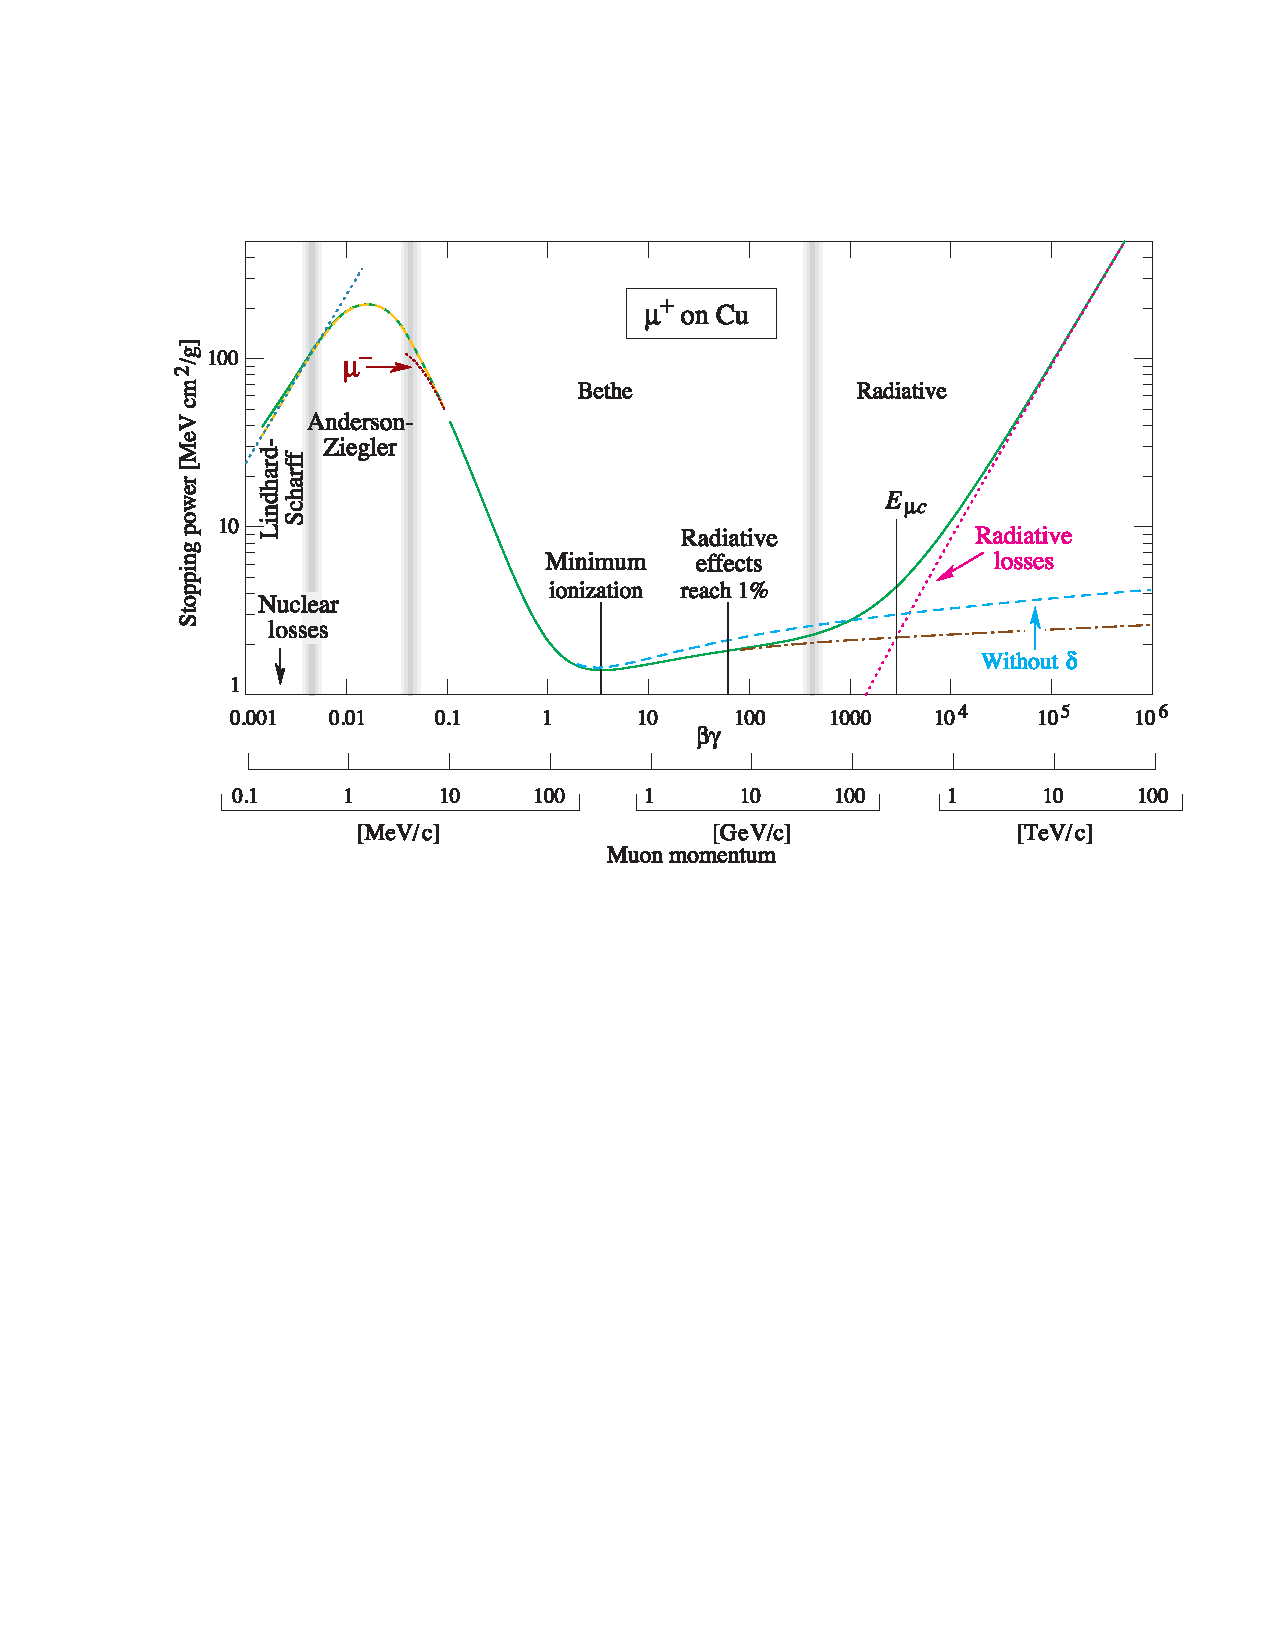
\includegraphics[scale=0.7]{./input/bethe.pdf}\caption{Energieverlust pro Strecke (Stopping power) aufgetragen gegen den Impuls eines Muons. Der Verlust durch Ionisation findet in einem Bereich von 10~Mev und 100~GeV statt\cite{Passage_through_matter}.}\label{fig:bethe}
\end{figure}
Um diesen Mittelwert ist der Energieverlust nach der Landau-Verteilung verteilt.
\begin{figure}
\centering
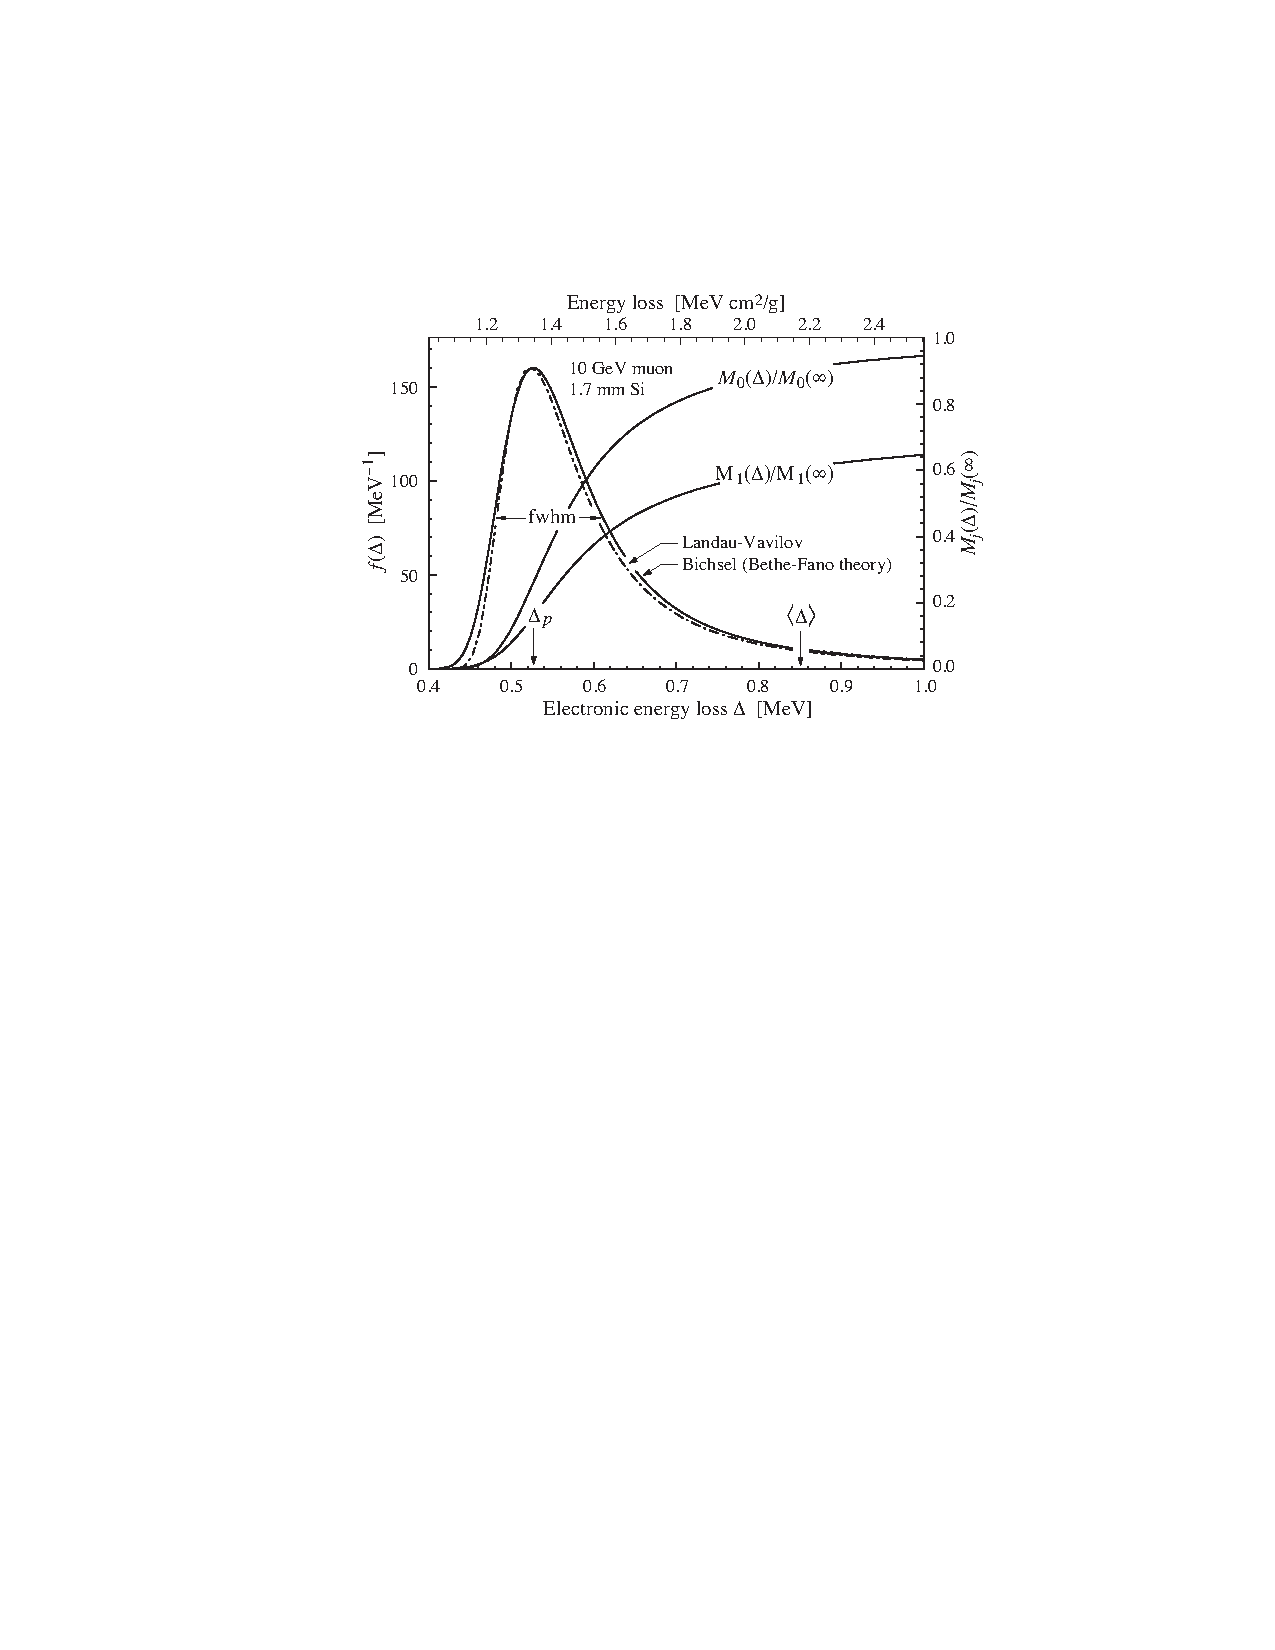
\includegraphics[]{./input/landau.pdf}\caption{Landau-Verteilung des nach Bethe-Bloch berechneten Energieverlusts.\cite{Passage_through_matter}}\label{fig:landau}
\end{figure}
\subsection{Elektronen und Photonen}
Photonen und Elektronen verlieren ihre Energie in Materie hauptsächlich durch Bremsstrahlung (Elektronen), und Paarerzeugung (Photonen). Weil ein Elektron durch Bremsstrahlung Photonen aussendet und ein Photon durch Paarerzeugung Elektronen erzeugt sind beide Vorgänge eng miteinander verbunden. Eine Materialkonstante, die eine wichtige Rolle spielt ist die Strahlungslänge $X_0$. Sie entspricht der Länge nachdem ein Elektron in Materie alles bis auf $1/e$ seiner Energie abgegeben hat. Gleichzeitig ist es $7/9$ der mittleren freien Weglänge eines Photons in diesem Material. Die aufeinander folgende Bremsstrahlung und Paarerzeugung von Photonen und Elektronen führt zu einer Teilchenkaskade, wie schematisch in Abb. \ref{fig:teilchen_kaskade} dargestellt.
\begin{figure}
\centering
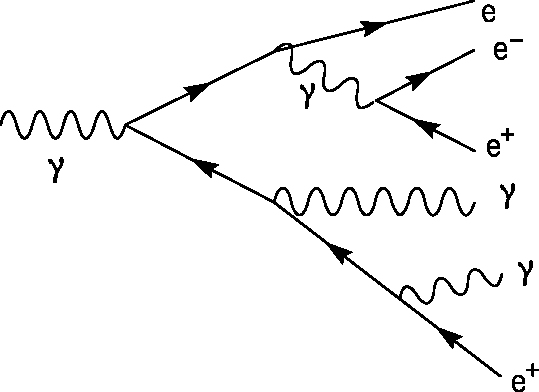
\includegraphics[]{./input/Schematic_of_a_particle_shower.pdf}\caption{Schematische Darstellung einer Elektromagnetischen Kaskade auch Schauer genannt\cite{emKaskade}.\comment{Wikipedia}}
\end{figure}

\section{Gas-Detektoren}
\subsection{Geiger-Zähler}
\subsection{Driftkammer}
\subsection{Time-Projection-Chamber}
text
\section{Teilchen Identifikation}
\subsection{Energieverlust}
\subsection{Time of Flight}
\subsection{Cherenkov Strahlung}
\subsection{Übergangsstrahlung}
text
\section{Cherenkov Detektoren}
text
\section{Halbleiter Detektoren}
\subsection{Halbleiter}
\subsection{Strahlungsschäden}
\subsection{Signalerzeugung}
\subsection{Silizium Detektor}
text
\section{Kalorimeter}
\subsection{Elektromagnetische Schauer}
\subsection{Hadronische Schauer}
\subsection{Sampling und homogene Kalorimeter}
\subsection{Energieauflösung}
text
